\documentclass[hyperref={pdfpagelabels=false}]{beamer} 

\usepackage[portrait]{sfocs-poster}
\usepackage{lipsum}

\usebackgroundtemplate{%
	% image as background
		\tikz\node[opacity=1] {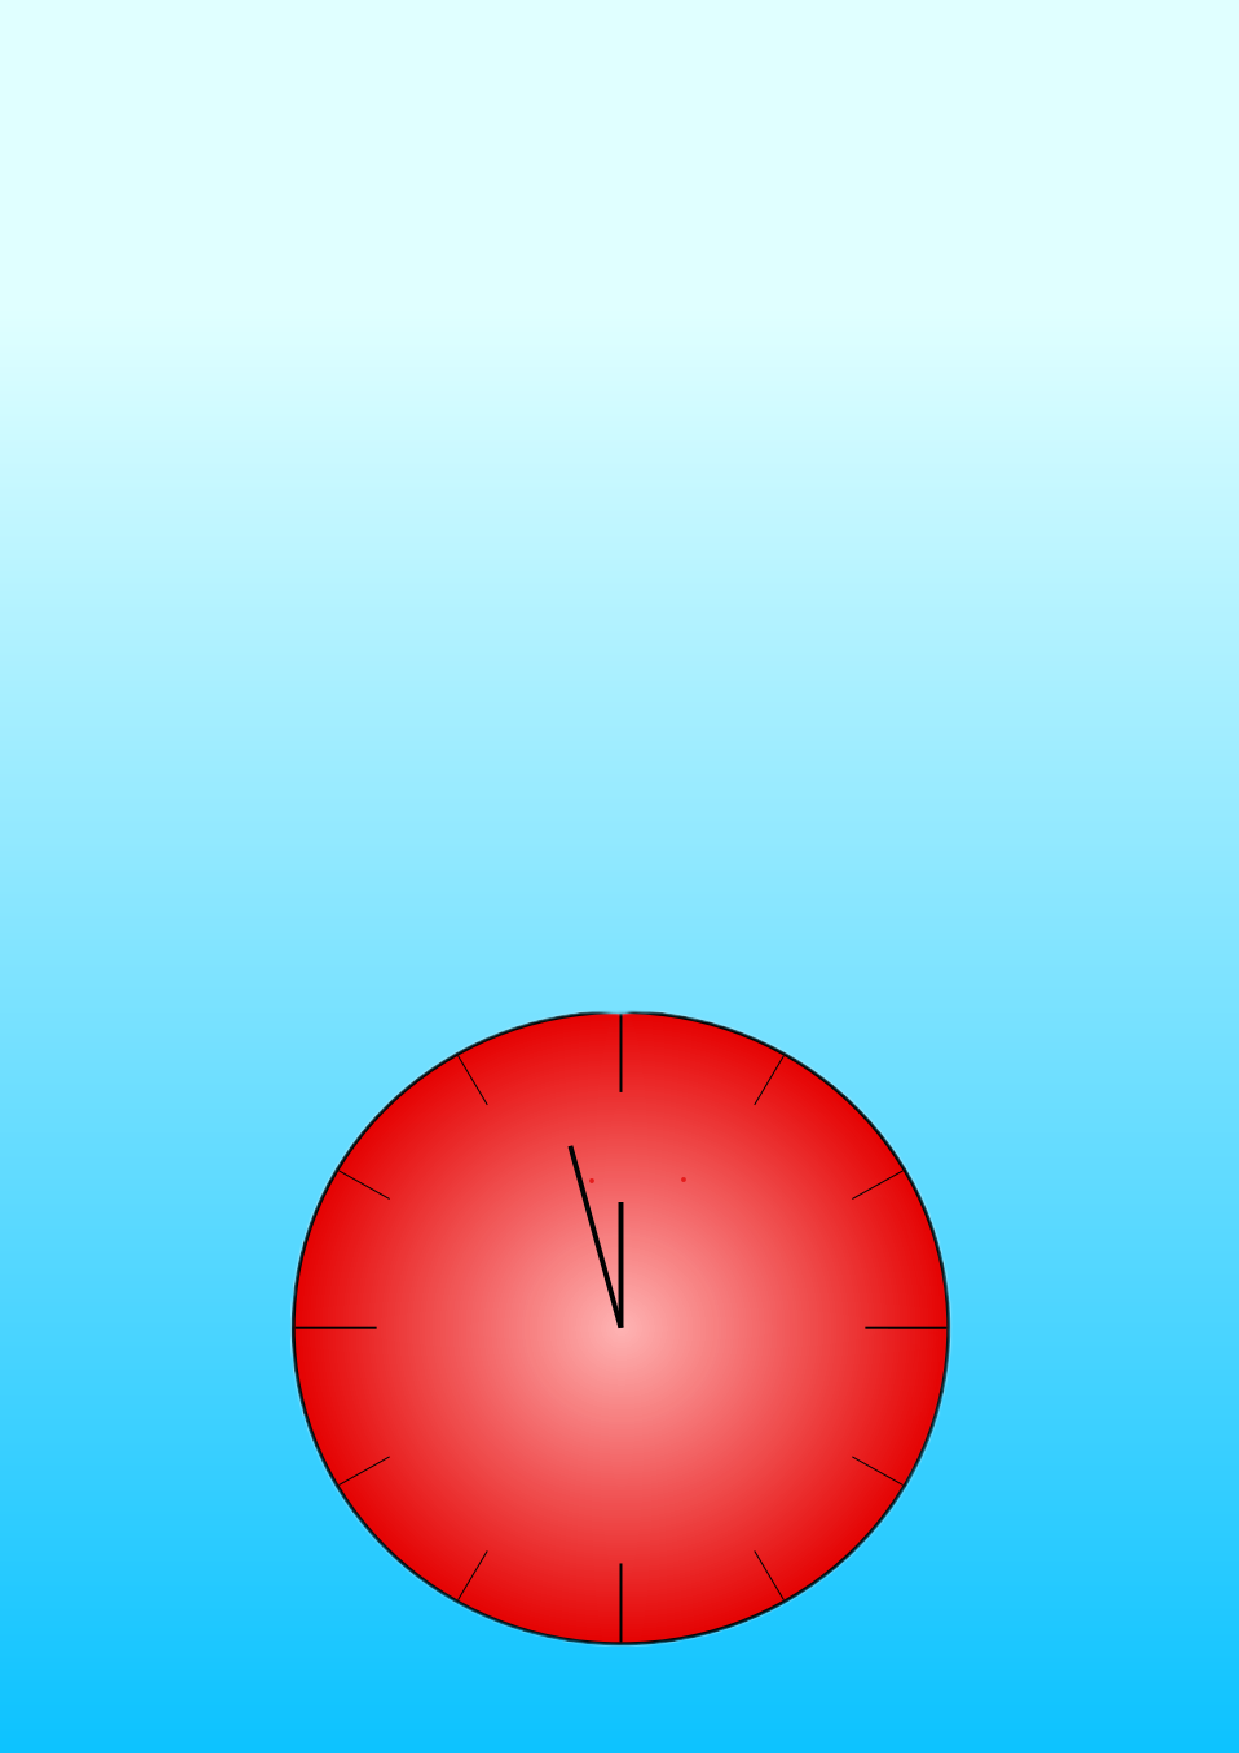
\includegraphics[height=\paperheight,width=\paperwidth]{img/pg}};
	% plain color 
	%\tikz[remember picture,overlay] \fill[game] (current page.north west) rectangle (current page.south east); 
}

%
% sample boxes 
% 
\tcbset{
        framedbox/.style={
					enhanced, fontupper=\large,left=.75cm,fonttitle=\LARGE,toptitle=.25cm,bottomtitle=.25cm,halign title=center
        },
}

\newtcolorbox{basebox}[3][]{framedbox,coltitle=#2,colback=#3,coltext=#2,title=#1,colframe=#3,sharp corners}
\newtcolorbox{baseroundedbox}[3][]{framedbox,colback=#3,colframe=#3,coltitle=#2,coltext=#2,title=#1,,rounded corners,arc=15pt}
\newtcolorbox{transparentbox}[4][]{framedbox, colback=#3,colbacktitle=#3,colframe=#3,coltitle=#2,coltext=#2,title=#1,frame style={color=#3},opacitybacktitle=#4,opacityback=#4,opacityframe=#4,opacityfill=#4}
\newtcolorbox{blankbox}{blanker,fontupper=\LARGE}


% draw a grid
%\beamertemplategridbackground[1cm]

\begin{document}

\begin{frame}

	\begin{textblock}{45}(2,1)
		\begin{blankbox}
			
\includegraphics[width=1000pt]{img/gamename.png} \\\hspace*{\fill} \\ \\\hspace*{\fill}

			\huge{You are faced with four areas in chaos stricken by a horrible pandemic. Citizen's lives and the urban resources are at stake! Appointed as the governor, it's your job to save as many lives as possible with only limited amount of critical resources and control points.}
		\end{blankbox}
	\end{textblock}

4	\begin{textblock}{30}(86,91)
		\begin{blankbox}
			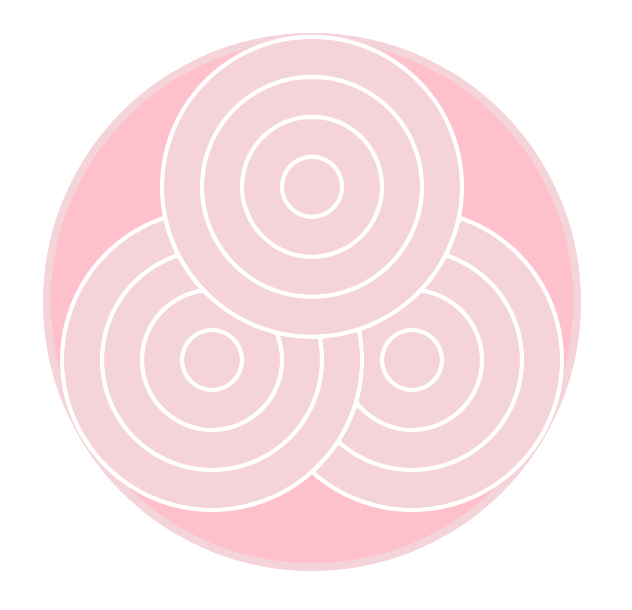
\includegraphics[width=250pt]{img/Teamlogo.png}

		\end{blankbox}
	\end{textblock}

	\begin{textblock}{20}(39,55.5)
		\begin{blankbox}
\centering
			\Huge MINIMALISM

\vspace{1cm}

			SIMPLICITY
\vspace{1cm}

ENTERTAINMENT
		\end{blankbox}
	\end{textblock}



	% #1: box width 
	% #2 #3: coordinates on percent 
\begin{textblock}{45}(5,37)
		\begin{blankbox}
	
			\huge{You are faced with four areas in chaos stricken by a horrible pandemic. Citizen's lives and the urban resources are at stake! Appointed as the governor, it's your job to save as many lives as possible with only limited amount of critical resources and control points.}
		\end{blankbox}
	\end{textblock}
	\begin{textblock}{90}(5,35)
		\begin{baseroundedbox}[]{black}{white}
			\begin{columns}
			\Large{	\begin{column}{0.55\columnwidth}
					Brief Instructions On The Game \\\hspace*{\fill} \\

					CP: Control Points\\
					CR: Critical Resources\\
					\begin{multicols}{2}
						\begin{itemize}
							\item Health Threat Drop: The dis-alarmed Health threat level
							\item Citizen Trust: The faith citizens in an area have in its governor
							\item External Safety: The safety guaranteed of the personnel and material inflow
							\item Disposable Money: The maximum financial aid offered to concerned institute
						\end{itemize}
					\end{multicols}
				\end{column}
				\begin{column}{0.5\columnwidth}
					\centering
					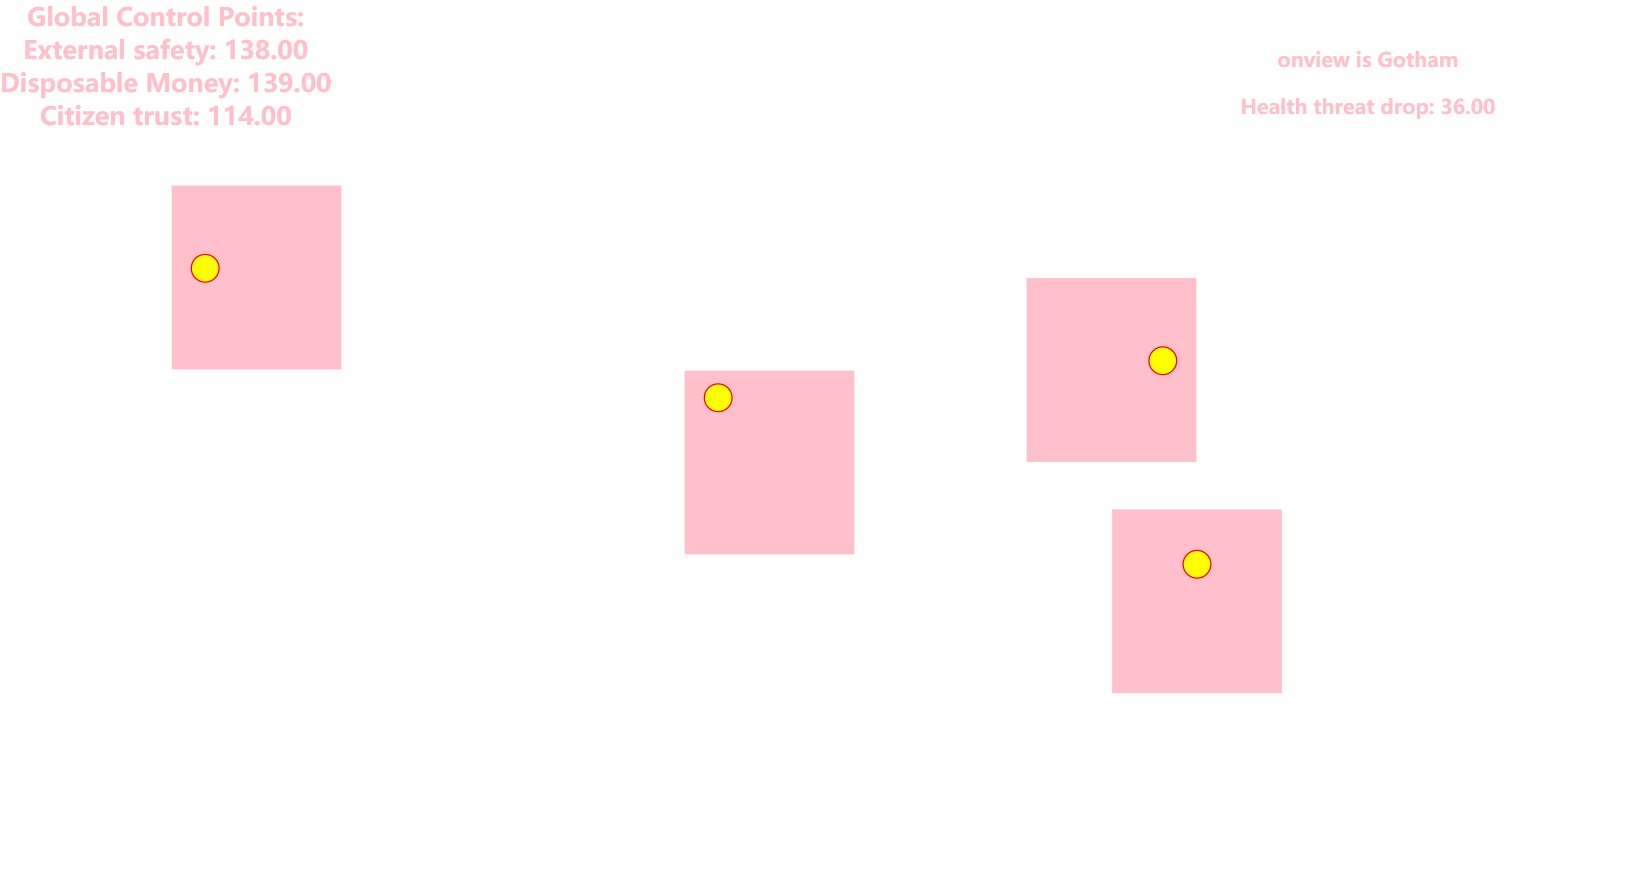
\includegraphics[width=0.9\columnwidth]{img/WechatIMG1131}
				\end{column}}
			\end{columns}

		\end{baseroundedbox}
	\end{textblock}
	
	\begin{textblock}{50}(25.5,70)
		% no title provided, extra parameter is opacity in [0,1] 		
		\begin{transparentbox}{white}{red}{.2}
				\centering \vspace{.25cm}
				\huge\textbf{Main Appeal}\vspace{1cm}

\begin{itemize}\itemsep .85cm
			\item Highly Customized User Control

				\item Simple yet ingenious Operation

				\item Minimalist User Interface

				\item  Diverse Gaming Modes
\end{itemize}       	 
		\end{transparentbox}
	\end{textblock} 

	% option [0,1] means box anchor is bottom left	
	\begin{textblock}{80}[0,1](1,100)
		\logos[light]
	\end{textblock}

	% option [1,1] means box anchor is bottom right	
	\begin{textblock}{30}[1,1](94,27)
		\begin{blankbox}
			\huge\textbf{{THREE TO ONE:}} \\\hspace*{\fill} \\
			\Large{Zining Wang (C)}\\ 
			Yifan Jia  \\
			Qiao Liu \\\hspace*{\fill} \\
			Our attention to the current affairs has inspired the game. Now you can be the protagonist and savior. \\\hspace*{\fill} \\\large{Good Luck!}
			
		\end{blankbox}
	\end{textblock}

	\begin{textblock}{10}(10,70)
		\begin{blankbox}
			\centering
			
\includegraphics[height=400pt]{img/ai97b-ej97b.png}
		\end{blankbox}
	\end{textblock}

	\begin{textblock}{10}(80,70)
		\begin{blankbox}
			\centering
			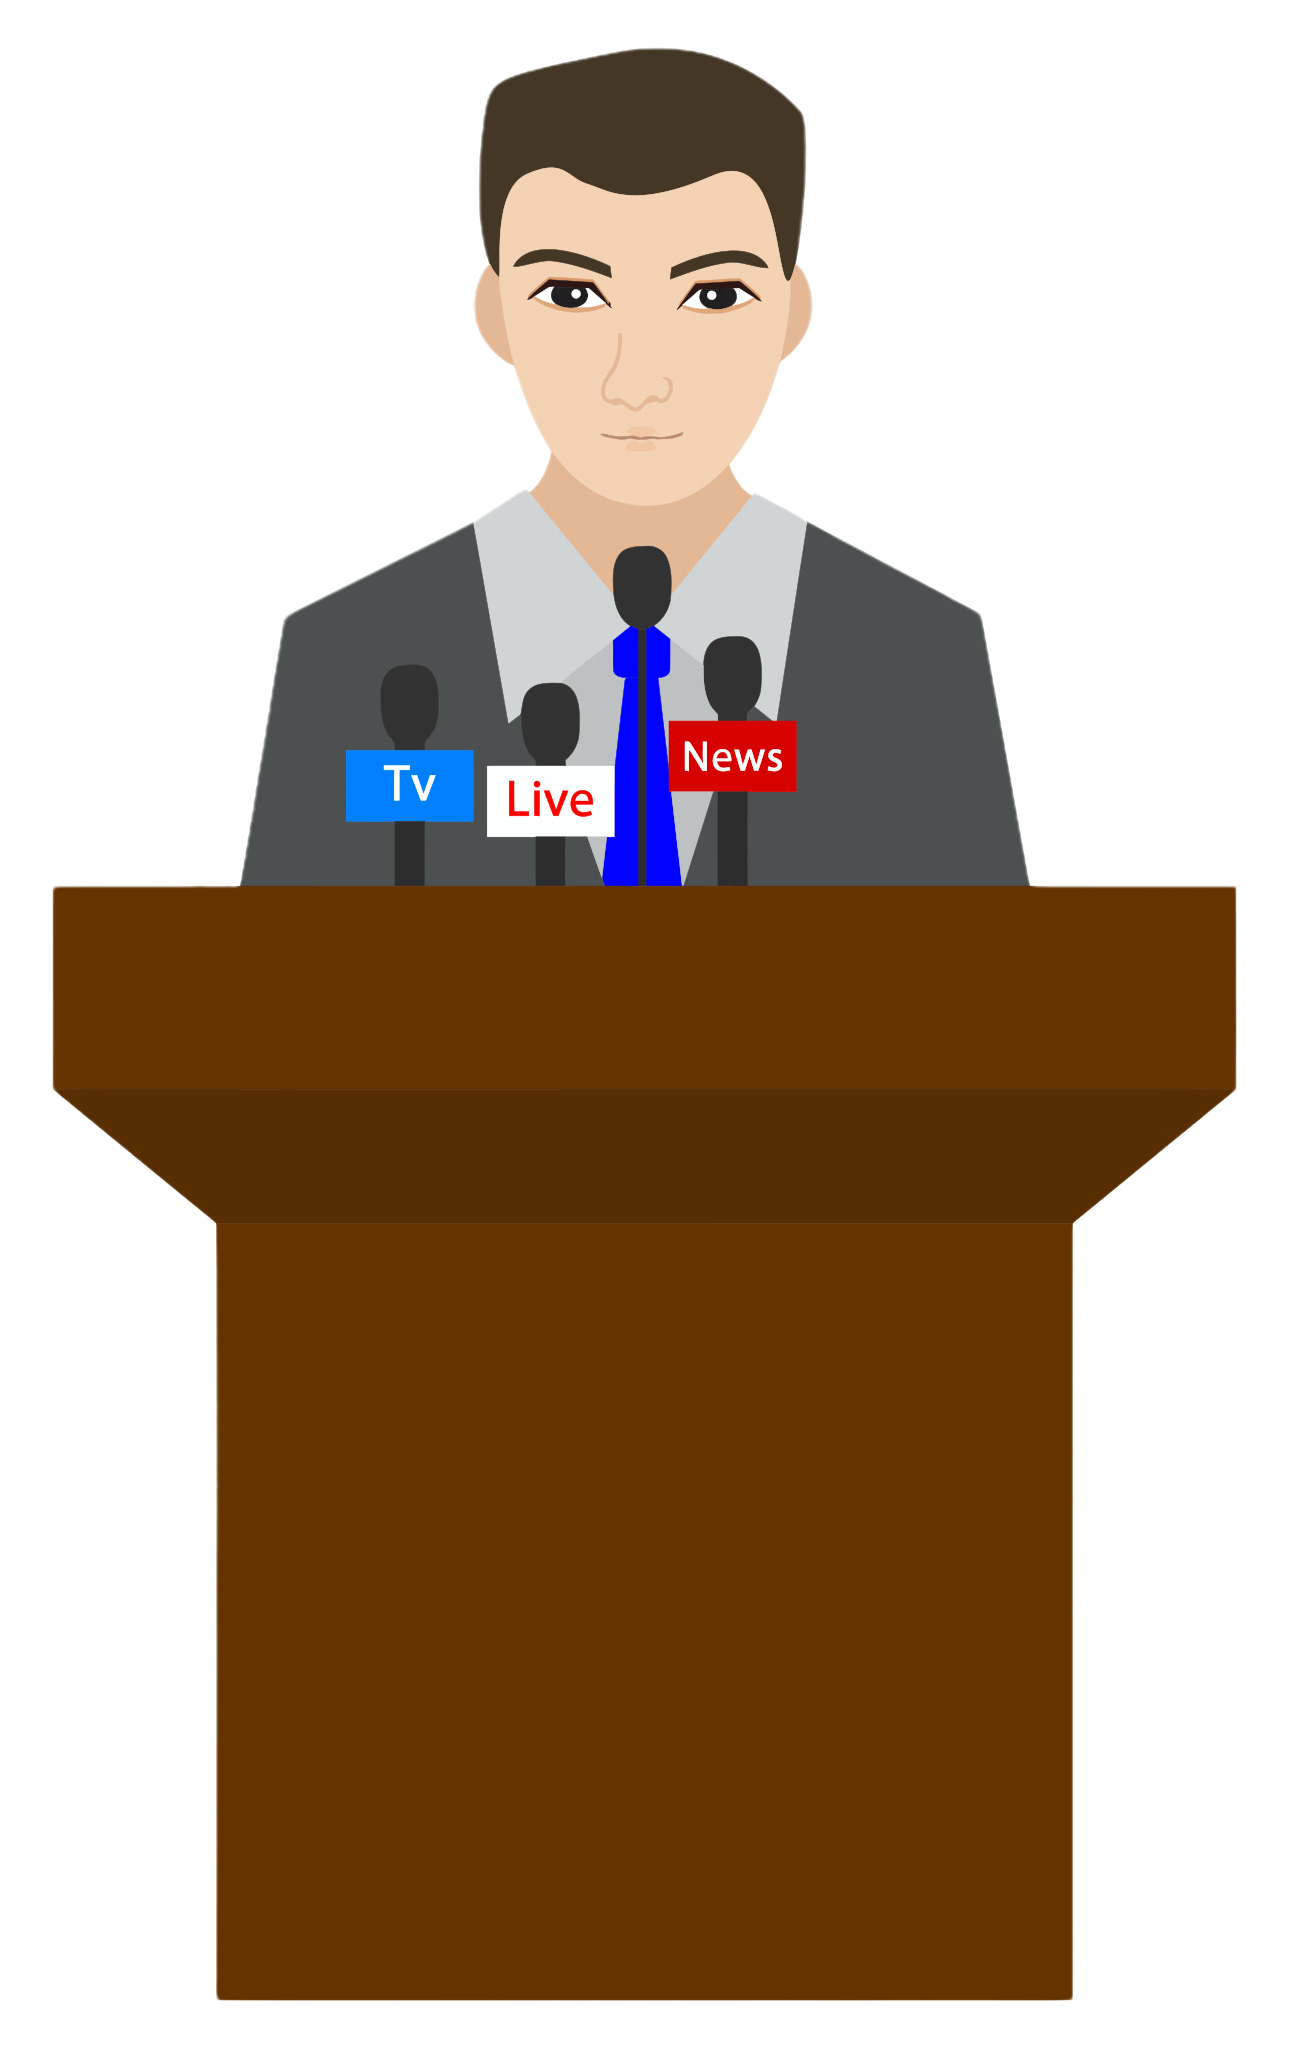
\includegraphics[height=400pt]{img/arn28-kj5eh.png}
		\end{blankbox}
	\end{textblock}


\end{frame}

\end{document}

transparent box 
larger title font 
no gradient 
plain box
